\chapter{xHCI Stack Implementation}

The structure of the xHCI driver is quite straightforward, as it tries to fit
into the scheme of how hardware and the rest of HelenOS works. We decided to
use the existing library \lib{libusbhost} to reduce code duplication with
other HC drivers. IT came out that this library need a lot of changes to
support us in this goal, but that's for chapter \ref{usb-refactoring}.

The USB host controller driver using \lib{libusbhost}, xHCI included, serves as
a connecting layer between the hardware and library, and exposes its bus
interface.

\begin{figure}[h]
	\centering
	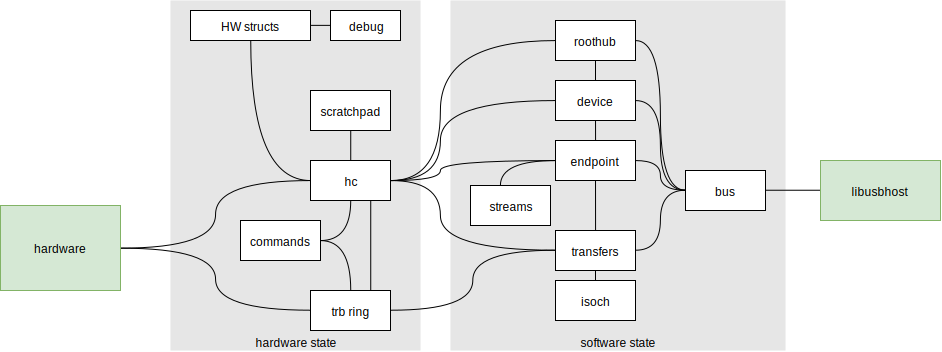
\includegraphics[width=0.8\textwidth]{xhci-architecture}
	\caption{The modules of xHCI driver}
\end{figure}

The scheme is not at all strict, we're in a C world, there are dependencies
almost everywhere -- take it as an informal overview to get an idea.

The whole driver can be split into two parts. The left one takes care about the
hardware perception on what's going on, the right one is about managing the
software structures and memory.

We start with describing the modules in the hardware part, as their
functionality is clear. Their order follows the order in which they were
implemented.

\section{HW structs}

% TODO: Explain that this one is really simple, and just mirrors the structures
% hardware use.

\section{Debug}

% TODO: Describe that we used it during debugging to check what we're doing.

\section{TRB ring}

% TODO @aearsis: explain the TRB rings, what they do and how they're
% implemented (ْ±2 pages, bore the reader to death right now!)
\subsection{Purpose}
\subsection{Implementation}

\section{Scratchpad}

% TODO: Anyone please explain these. The only interesting part is how the
% number of buffers are split weird and how we needed several attempts to get
% it right :)

\section{Commands}

% TODO @dzejrou or @petr: Explain why commands are needed and the basic
% structure of the subsystem
\subsection{Purpose}
\subsection{Implementation}

% TODO @petr: Show off with the inline syntax

\subsubsection{Aborting commands}

% TODO @aearsis: Explain the arcane magic behind aborting commands.

\section{Host controller module}

% TODO: This will be harder, this one is a mix of what didn't fit anywhere else.
% Ideas:
% - event handling
% - context management
% - extcap parsing
% - register access macros

\section{Roothub}

% TODO: Explain why we do not have virthub. Who remembers the reasons?
% Otherwise it just uses libusb/port to do the interesting work.

\section{Transfers}

% TODO @salmelu (probably?): Write something about it.

\subsection{Isochronous transfers}

% TODO @salmelu: Copy that from the wiki :)

\section{Bus module}

% TODO: After the device will be split, will there be anything interesting to write about?

\subsection{Device}

% TODO: Enumeration, device context

\subsection{Endpoint}

% TODO: Contexts, rings

\subsection{Streams}

% TODO @salmelu: Noone else understands that now.
